\documentclass[runningheads]{llncs}
\usepackage{graphicx}
\usepackage{booktabs}
\usepackage{amsmath}
\usepackage[hidelinks]{hyperref}
\usepackage{xurl}
\usepackage{xcolor}
\usepackage{multirow}
\hypersetup{
  pdftitle={Automating the Detection of Misleading Design Rationale Generated by Large Language Models: An Empirical Evaluation of a Verifier Agent},
  pdfauthor={Vo Khoi Nguyen, Duong Dinh Tri, Nguyen Ngoc Nha Vy, Tran Dinh Hai Phung, Nguyen Hieu Thong}
}
\newcommand{\todo}[1]{\textcolor{red}{\textbf{[TODO: #1]}}}
\begin{document}
\sloppy
\title{Automating the Detection of Misleading Design Rationale Generated by Large Language Models: An Empirical Evaluation of a Verifier Agent}
\author{Vo Khoi Nguyen\inst{1} \and Duong Dinh Tri\inst{1} \and Nguyen Ngoc Nha Vy\inst{1} \and Tran Dinh Hai Phung\inst{1} \and Nguyen Hieu Thong\inst{1}}
\authorrunning{Nguyen et al.}
\titlerunning{Detecting Misleading LLM-Generated Design Rationale}
\institute{FPT University, Ho Chi Minh City Campus, Vietnam \\
\email{khoinguyen.vo910@gmail.com, dinhtri11012005@gmail.com, nhaua123@gmail.com, phungtr59@gmail.com, hieuthong15082005@gmail.com}}
\maketitle
\begin{abstract}
Large language models (LLMs) are increasingly used to generate \emph{design rationale} (DR) --- the justification for why a software architecture decision is appropriate. A recent large-scale study by Zhou et al.\ evaluated three LLM prompting strategies for DR generation against a benchmark of 100 real-world architecture problems and found that, across those three prompting strategies, between 1.59\% and 3.24\% of generated argument statements were \emph{Misleading}: confidently stated but factually incorrect. Crucially, that evaluation relied entirely on manual labeling by four human experts, with no automated mechanism to flag unreliable rationale before it reaches a developer. We present, to our knowledge, the first empirical evaluation of an LLM-based \emph{Verifier Agent} that automatically audits LLM-generated DR against the original problem context, replicating Zhou et al.'s four-category labeling scheme (Insightful, Helpful, Uncertain, Misleading) at the granularity available in their public ground truth --- per-DR category presence rather than per-argument labels --- without human intervention. Using Gemini 3.1 Flash-Lite as the verifier backbone, we evaluate three verifier prompting strategies (zero-shot, chain-of-thought, few-shot) and, for the chain-of-thought strategy, an additional context-withheld condition, totaling 1{,}200 verifier predictions against Zhou et al.'s public ground truth. We find that, for the chain-of-thought verifier, supplying the original architecture-problem context is the single largest driver of performance, nearly tripling Misleading-detection F1 (0.056 $\rightarrow$ 0.152) and raising macro F1 from 0.406 to 0.608; differences among prompting strategies (all with context supplied) are comparatively small (macro F1 0.608--0.625). We report per-category precision/recall/F1, Cohen's Kappa against human labels, and an error analysis by DR length and architecture-decision type, and discuss why Misleading-argument detection remains substantially harder than detecting Insightful or Helpful content.
\keywords{Design Rationale \and Large Language Models \and LLM-as-a-Judge \and Software Architecture \and Hallucination Detection \and Empirical Software Engineering}
\end{abstract}
\section{Introduction}
\label{sec:intro}
Design rationale (DR) --- the explicit justification for why a particular architecture decision was chosen over its alternatives --- is widely recognized as essential architectural knowledge, yet it is chronically under-documented in practice because writing it down is time-consuming and easy to defer \cite{zhou2025llm}. Large language models (LLMs) have recently been proposed as a way to close this gap by automatically synthesizing DR from the surrounding problem description and the decision that was made \cite{zhou2025llm,dhar2024llm,diazpace2024archmind}.
Zhou et al.\ conducted the most comprehensive evaluation of this idea to date \cite{zhou2025llm}, benchmarking three LLM prompting strategies for DR generation (zero-shot, chain-of-thought, and an LLM-agent pipeline) across five model families on 100 real architecture problems mined from Stack Overflow, GitHub, and technical discussions. Each generated DR was manually decomposed into individual arguments and labeled by four human experts into one of four categories, adapted from prior work on information quality: \emph{Insightful} (correct and central to the decision), \emph{Helpful} (correct but secondary), \emph{Uncertain} (unverifiable from the available context), and \emph{Misleading} (confidently stated but factually wrong). Across their three prompting strategies, \textbf{1.59\%--3.24\% of generated arguments were Misleading} --- the most dangerous category, since a confidently wrong architectural justification can misdirect an engineer who trusts it. Critically, Zhou et al.\ note that this labeling process was entirely manual: no automated mechanism exists to flag a Misleading argument before a generated DR is shown to a developer.
This gap motivates our contribution. Rather than proposing a new DR-generation technique, we ask a narrower and, we argue, more immediately actionable question: \emph{can an LLM itself be used as an automatic Verifier to catch Misleading arguments in already-generated DR, replacing the manual labeling step in Zhou et al.'s pipeline?} This follows the broader ``LLM-as-a-judge'' paradigm, in which a language model is used to evaluate the output of another (or the same) model against human-aligned criteria \cite{zheng2023judging}, and is conceptually related to the general problem of hallucination detection in LLM outputs \cite{huang2025survey,farquhar2024semantic,manakul2023selfcheckgpt} --- with the difference that our ``hallucinations'' are domain-specific factual errors about a concrete, verifiable architecture context rather than open-domain claims.
We pose two research questions:
\begin{description}
\item[RQ1] How accurately can an automated Verifier Agent detect Misleading design rationale, compared to the human-expert ground truth established by Zhou et al.?
\item[RQ2] Does supplying the Verifier Agent with the original problem context (as opposed to judging the DR in isolation) meaningfully change its ability to catch Misleading arguments, and how does this compare across different verifier prompting strategies?
\end{description}
To answer these questions we build a Verifier Agent that takes the original architecture problem and decision (but \emph{not} the human-written reference DR, to avoid leaking the answer key) together with an LLM-generated DR, segments the DR into individual arguments, and labels each one using Zhou et al.'s four-category taxonomy, with a supporting justification and an evidence quote drawn from the original context. We evaluate this agent on the publicly released LLM4DR dataset \cite{zhou2025llm}, using the DR generated by GPT-4-0613 (the strongest generator in Zhou et al.'s study) under all three of Zhou et al.'s generation strategies (zero-shot, chain-of-thought, and LLM-agent), for a total of 300 DRs. We evaluate three verifier prompting strategies --- zero-shot, chain-of-thought, and few-shot --- each with the original context supplied, and additionally run the chain-of-thought strategy with the original context withheld to isolate its contribution. This yields four experimental conditions and 1{,}200 verifier predictions in total, all produced by a single fixed model (Gemini 3.1 Flash-Lite, temperature 0) to keep the comparison scientifically controlled. We note this design measures the context-availability effect only for the chain-of-thought verifier; it does not establish whether context matters equally for zero-shot or few-shot prompting (see Limitations).
\paragraph{Contributions.} (1) We present, to our knowledge, the first empirical evaluation of an LLM-as-Verifier approach specifically for catching Misleading LLM-generated architecture design rationale. (2) We provide an ablation isolating the effect of prompting strategy from the effect of context availability for the chain-of-thought verifier, showing that context availability dominates the choice of prompting strategy. (3) We report an honest, non-overclaiming assessment: our Verifier Agent detects a substantial portion of Misleading arguments (recall 0.350--0.550 depending on prompting strategy, all with context) but at low precision (0.097--0.118 with context), and we analyze \emph{why} through an error analysis by DR length and architecture-decision type. (4) We release our prompts, evaluation code, and full API call logs to support reproducibility.
\section{Related Work}
\label{sec:relwork}
\subsection{LLM-Generated Design Rationale and Architectural Knowledge}
Zhou et al.\ \cite{zhou2025llm} is the direct baseline for this work: they evaluate zero-shot, chain-of-thought, and LLM-agent prompting strategies across five LLMs for generating DR on 100 real architecture problems, introducing the Insightful\allowbreak/Helpful\allowbreak/Uncertain\allowbreak/Misleading (IHUM) taxonomy we adopt, and releasing the LLM4DR dataset and human-expert labels we build on. Dhar et al.\ \cite{dhar2024llm} conduct a complementary exploratory study asking whether LLMs can generate architectural design decisions themselves (rather than just the rationale for a decision made by a human), finding LLMs can produce plausible decisions but with notable gaps against expert judgment. D\'{i}az-Pace et al.\ \cite{diazpace2024archmind} propose an LLM-based assistant, ArchMind, that helps novice architects capture and critique architecture decisions interactively; unlike our work, their LLM acts as a co-author rather than an independent auditor of already-generated content.
\subsection{LLM-as-a-Judge}
Our Verifier Agent instantiates the broader ``LLM-as-a-judge'' paradigm formalized by Zheng et al.\ \cite{zheng2023judging}, who show that strong LLMs can approximate human preference judgments on open-ended chatbot responses with reasonably high agreement. We apply this idea to a much narrower, domain-specific setting --- verifying factual claims about a concrete, given architecture context --- rather than open-ended preference judgment, which we argue is an easier and more falsifiable task for an LLM judge, since claims can in principle be checked against the supplied context rather than relying on the judge's general knowledge or taste.
\subsection{Hallucination Detection in LLMs}
The Misleading category in Zhou et al.'s taxonomy is, in effect, a domain-specific instance of LLM hallucination: content that is fluent and confident but not supported by (or contradicted by) the available evidence. Huang et al.\ \cite{huang2025survey} provide a comprehensive taxonomy and survey of hallucination detection and mitigation techniques. Two representative detection techniques illustrate the range of approaches: Farquhar et al.\ \cite{farquhar2024semantic} detect hallucinations via semantic entropy over sampled generations without requiring external knowledge sources, while Manakul et al.\ \cite{manakul2023selfcheckgpt} propose SelfCheckGPT, a zero-resource, black-box technique that checks response consistency across resamples. Our setting differs from both in an important way: because the Verifier Agent is given the original problem/decision context directly, detection is closer to a grounded fact-checking task than to the resource-free hallucination detection these works target, which is precisely why we hypothesize --- and find supporting evidence in Section~\ref{sec:results} --- that supplying context should matter a great deal.
\subsection{LLMs for Requirements and Quality Classification}
Closer to our per-argument non-functional-requirement (NFR) tagging (Section~\ref{sec:methodology}), Alhoshan et al.\ \cite{alhoshan2025requirements} evaluate generative LLMs on requirements classification tasks, including NFR categorization on the PROMISE dataset; we note this is currently an unpublished preprint. Our work differs in applying LLM-based classification not to standalone requirements statements but to individual arguments embedded within a generated design rationale, where correctness must additionally be checked against a specific problem context rather than classified in isolation.
\section{Methodology}
\label{sec:methodology}
\subsection{Problem Framing: Per-DR Aggregate Verification}
Zhou et al.'s publicly released ground truth records, for each generated DR, how many of its constituent arguments were labeled Insightful, Helpful, Uncertain, and Misleading by human experts (an aggregate \emph{count} per category, per DR) --- it does not release the underlying per-argument text-to-label mapping. To evaluate our Verifier Agent at a granularity that matches this available ground truth, we adopt a \emph{per-DR aggregate} design: the Verifier Agent independently segments a given DR into its own set of arguments and labels each one, and we compare the \emph{presence} of each category in the Verifier's output against the \emph{presence} of that category in the human ground truth (i.e., whether the human-labeled count for that category is greater than zero), rather than attempting a one-to-one argument alignment that the public dataset does not support. We operationalize this as four independent binary classification problems (one per IHUM category, per DR): did this DR contain at least one argument of category $X$, according to the Verifier, and according to the human experts?
\subsection{Verifier Agent Design}
The Verifier Agent takes two inputs: (1) the \emph{original architecture problem and decision} exactly as it appeared in the source Stack Overflow/GitHub/discussion thread (the same context a human expert would have used to write the reference DR), and (2) an \emph{LLM-generated DR} to audit. Critically, the Verifier is \textbf{not} shown the human-written reference DR from Zhou et al.'s dataset, since that text was the basis on which the ground-truth IHUM labels were originally assigned by the human annotators, and exposing it to the Verifier would leak the answer key.
Given these inputs, the Verifier Agent is instructed to: (a) segment the generated DR into discrete arguments (roughly one claim or reason per sentence or bullet point); (b) for each argument, assign one of the four IHUM labels, using only the supplied original context as evidence; (c) provide a short justification and, where possible, a verbatim evidence quote from the original context supporting or contradicting the argument; and (d) tag the argument with zero or more of five non-functional-requirement (NFR) categories (performance, security, maintainability, scalability, reliability) that it concerns, if any. Zhou et al.'s public ground truth does not include per-argument NFR labels, so we cannot score NFR tagging against a gold standard; we collect it as part of the Verifier's output and release it in our artifact to support future qualitative analysis and NFR-aware filtering, but we do not evaluate it quantitatively in this paper. The full instruction prompt is included in our released artifact. Output is constrained to a strict JSON schema, which we parse deterministically; per-DR category counts are obtained by aggregating the labels across all extracted arguments for that DR.
\subsection{Verifier Prompting Strategies (Ablation Axis 1)}
We evaluate three prompting strategies for the Verifier Agent itself, orthogonal to (and not to be confused with) the DR-\emph{generation} strategies used by Zhou et al.\ (Section~\ref{sec:expsetup}):
\begin{description}
\item[Zero-shot] The task description and output schema only, with no worked example and no explicit reasoning instruction.
\item[Chain-of-thought (CoT)] The zero-shot prompt augmented with an instruction to internally reason step by step (list every argument, check each against the context, then decide) before producing the final JSON, with the intermediate reasoning suppressed from the output.
\item[Few-shot] The CoT prompt augmented with one hand-written, synthetic worked example (a message-queue architecture decision, unrelated to any problem in the 100-problem benchmark) demonstrating the full input/output format, including one example of each of the four IHUM labels.
\end{description}
\subsection{Context Availability (Ablation Axis 2)}
To isolate the contribution of the original problem context, we additionally run the CoT prompting strategy under a \emph{context-withheld} condition, in which the Verifier Agent receives only the generated DR (no original architecture problem or decision) and is explicitly told to label any unverifiable claim as Uncertain rather than guessing. Comparing this against the context-available CoT condition directly measures how much grounding in the original problem contributes to Verifier accuracy, addressing RQ2.
\subsection{Use of AI in Manuscript Preparation}
Beyond the Verifier Agent under study, an AI assistant (Claude, Anthropic) was used to help draft portions of this manuscript's prose --- including sections of the Introduction, Results narrative, Discussion, and Limitations --- from the authors' experimental results, logs, and notes, under direct author supervision. All experimental design, code, and numerical results were produced by the authors' pipeline (Sections~\ref{sec:methodology}--\ref{sec:expsetup}) and independently verified by the authors against the underlying data before inclusion. This use goes beyond AI-assisted copy editing as defined by Springer Nature's authorship policy and is disclosed here accordingly; the authors reviewed, verified, and take full accountability for the final content of this manuscript.
\section{Experimental Setup}
\label{sec:expsetup}
\subsection{Dataset}
We use the publicly available LLM4DR dataset released by Zhou et al.\ \cite{zhou2025llm} (\url{https://github.com/Eric0052/LLM4DR}), which contains 100 real-world architecture problems sourced from Stack Overflow, GitHub, and technical discussion threads, each paired with a human-expert-written reference DR and IHUM labels for DR generated under three prompting strategies --- \emph{zero-shot}, \emph{chain-of-thought}, and an \emph{LLM-agent} pipeline --- across five LLM families. We use the DR generated by \texttt{GPT-4-0613}, the strongest generator model reported in Zhou et al., under all three of their generation strategies, yielding $100 \times 3 = 300$ DRs as the input to our Verifier Agent. We deliberately do not collect any additional data: the ground-truth IHUM counts we evaluate against are exactly those released by Zhou et al.
\subsection{Verifier Model and Reproducibility}
The Verifier Agent is implemented with the Gemini API, using \texttt{gemini-3.1-flash-lite} at temperature $0$ for all 1{,}200 calls, chosen for cost reasons (the model is available under Google's free tier) and to enable an easily reproducible, zero-training pipeline. To guard against silent model drift --- Gemini model aliases can be transparently repointed to a different underlying model by the provider --- we log the SDK-reported \texttt{model\_version} field for every successful call and confirm that all 1{,}200 predictions used in our final analysis resolved to the same concrete model version. Every API call (prompt, raw response, latency, and any error) is logged to a persistent JSONL audit trail; on transient failures (e.g., rate-limit or quota errors), calls are retried with exponential backoff, and a resume mechanism ensures that once a given (problem, generation strategy, verifier variant, context condition) combination succeeds, it is never re-queried, preventing duplicate or inconsistent entries in the final dataset.
\subsection{Experimental Conditions}
Combining the three verifier prompting strategies (Section~\ref{sec:methodology}) with the context-availability ablation yields four experimental conditions, each evaluated on all 300 DRs, for $4 \times 300 = 1{,}200$ total verifier predictions:
\begin{enumerate}
\item Zero-shot, with context
\item Few-shot, with context
\item Chain-of-thought, with context
\item Chain-of-thought, without context
\end{enumerate}
\subsection{Metrics}
For each IHUM category and each experimental condition, we report \textbf{precision}, \textbf{recall}, and \textbf{F1} for the binary ``category present in this DR'' task described in Section~\ref{sec:methodology}, together with \textbf{Cohen's Kappa} against the human-expert ground truth to account for chance agreement, and \textbf{macro-F1} averaged across the four categories. As a secondary, more fine-grained view, for the context ablation we also report the \textbf{mean absolute error (MAE)} between the Verifier's predicted per-category argument \emph{count} and the human-expert count for that category. We focus our discussion primarily on the \textbf{Misleading} category, since it is both the rarest (present in only 6.7\% of DRs in our sample) and the highest-stakes to catch.
\section{Results}
\label{sec:results}
\subsection{RQ2: Effect of Context Availability}
Table~\ref{tab:context-ablation} reports per-category performance for the chain-of-thought verifier, with and without the original architecture-problem context. Supplying context produces a substantial improvement across every category except Uncertain, and the effect is largest exactly where it matters most: \textbf{Misleading-detection F1 increases from 0.056 to 0.152}, a nearly $3\times$ improvement, while macro-F1 rises from 0.406 to 0.608. The Insightful and Helpful categories improve primarily via recall (0.392$\rightarrow$0.993 and 0.507$\rightarrow$0.983 respectively): without context, the Verifier appears to systematically \emph{under}-predict these two categories, likely because it cannot confidently confirm an argument's correctness or centrality without something to check it against, and defaults toward Uncertain instead (Uncertain's without-context recall of 0.905 supports this interpretation, at the cost of very low precision, 0.210).
As a secondary, count-level view, mean absolute error (MAE) between the Verifier's predicted per-category argument count and the human-expert count moves in the same direction as F1 for three of the four categories: supplying context reduces MAE for Insightful (1.370$\rightarrow$1.223), Helpful (2.880$\rightarrow$1.713), and, most sharply, Uncertain (4.843$\rightarrow$0.947). Misleading is the exception: MAE slightly \emph{increases} with context (0.117$\rightarrow$0.330) even though F1 nearly triples. This is not a contradiction --- without context the Verifier almost never predicts Misleading at all (it defaults to Uncertain, as noted above), so its count error is small simply because both its prediction and the true count are usually close to zero; with context it predicts Misleading far more often, which raises both true and false positives and therefore count error, even as detection (F1) improves. This illustrates that MAE and F1 can disagree for a rare, low-precision category, and neither alone characterizes the Verifier's behavior on Misleading.
\begin{table}[t]
\centering
\caption{Context ablation: chain-of-thought (CoT) Verifier, with vs.\ without the original architecture-problem context ($n=300$ DRs per condition). P = precision, R = recall.}
\label{tab:context-ablation}
\small
\begin{tabular}{lccccccc}
\toprule
\multirow{2}{*}{Category} & \multicolumn{3}{c}{No context} & \multicolumn{3}{c}{With context} & \multirow{2}{*}{$\Delta$F1} \\
\cmidrule(lr){2-4} \cmidrule(lr){5-7}
 & P & R & F1 & P & R & F1 & \\
\midrule
Insightful  & 0.932 & 0.392 & 0.552 & 0.929 & 0.993 & 0.960 & +0.408 \\
Helpful     & 1.000 & 0.507 & 0.673 & 1.000 & 0.983 & 0.992 & +0.319 \\
Uncertain   & 0.210 & 0.905 & 0.341 & 0.215 & 0.667 & 0.326 & $-$0.015 \\
Misleading  & 0.062 & 0.050 & 0.056 & 0.097 & 0.350 & 0.152 & +0.096 \\
\midrule
\textbf{Macro F1} & \multicolumn{3}{c}{\textbf{0.406}} & \multicolumn{3}{c}{\textbf{0.608}} & \textbf{+0.202} \\
\bottomrule
\end{tabular}
\end{table}
\subsection{RQ1: Effect of Verifier Prompting Strategy}
Table~\ref{tab:prompt-ablation} compares the three verifier prompting strategies, all with context supplied. Overall macro-F1 is remarkably stable across strategies (0.608--0.625), indicating that, once context is available, the choice of prompting strategy is a second-order effect compared to context availability itself. For Misleading detection specifically, zero-shot achieves the highest recall (0.550) and few-shot the highest precision (0.118) and highest F1 (0.188); chain-of-thought is, perhaps counter-intuitively, the weakest of the three on this category (F1 0.152), which we discuss further in Section~\ref{sec:discussion}.
\begin{table}[t]
\centering
\caption{Verifier prompting-strategy comparison, all with context supplied ($n=300$ DRs per condition).}
\label{tab:prompt-ablation}
\footnotesize
\begin{tabular}{lccccccccc}
\toprule
\multirow{2}{*}{Category} & \multicolumn{3}{c}{Zero-shot} & \multicolumn{3}{c}{Few-shot} & \multicolumn{3}{c}{CoT} \\
\cmidrule(lr){2-4} \cmidrule(lr){5-7} \cmidrule(lr){8-10}
 & P & R & F1 & P & R & F1 & P & R & F1 \\
\midrule
Insightful & 0.929 & 0.986 & 0.956 & 0.929 & 0.982 & 0.955 & 0.929 & 0.993 & 0.960 \\
Helpful    & 1.000 & 0.990 & 0.995 & 1.000 & 0.993 & 0.997 & 1.000 & 0.983 & 0.992 \\
Uncertain  & 0.220 & 0.778 & 0.343 & 0.236 & 0.746 & 0.359 & 0.215 & 0.667 & 0.326 \\
Misleading & 0.115 & 0.550 & 0.190 & 0.118 & 0.450 & 0.188 & 0.097 & 0.350 & 0.152 \\
\midrule
\textbf{Macro F1} & \multicolumn{3}{c}{\textbf{0.621}} & \multicolumn{3}{c}{\textbf{0.625}} & \multicolumn{3}{c}{\textbf{0.608}} \\
\bottomrule
\end{tabular}
\end{table}
\subsection{Agreement with Human Experts}
Cohen's Kappa for the Misleading category is low across all conditions (0.053--0.092 with context; $-$0.004 without), indicating agreement only slightly above chance despite non-trivial recall. This is consistent with a Verifier that catches a real fraction of true Misleading arguments but also produces many false positives (65 false positives vs.\ 7 true positives for the CoT-with-context condition; Fig.~\ref{fig:confmat}), so raw recall alone overstates practical reliability. Kappa for Insightful is modest (0.041--0.064 with context) despite very high raw precision and recall (F1 up to 0.960), because its 92.7\% ground-truth base rate mechanically compresses the room for chance-corrected agreement. Helpful's ground-truth base rate is exactly 100\% (every DR in our sample contains at least one Helpful argument), which makes Cohen's Kappa mathematically degenerate for this category: with no true negatives possible, observed agreement and chance-expected agreement coincide algebraically, forcing Kappa to exactly 0.000 in every condition regardless of the Verifier's actual quality; we report it for completeness but treat it as uninformative rather than as evidence of weak agreement. Notably, this means Misleading's Kappa (0.053--0.092 with context) is numerically \emph{higher} than Insightful's, despite Misleading being by far the harder detection task on every other metric --- a reminder that raw Kappa values are not directly comparable across categories with very different ground-truth base rates, and should be read alongside precision/recall/F1 rather than in isolation.
\begin{figure}[t]
\centering
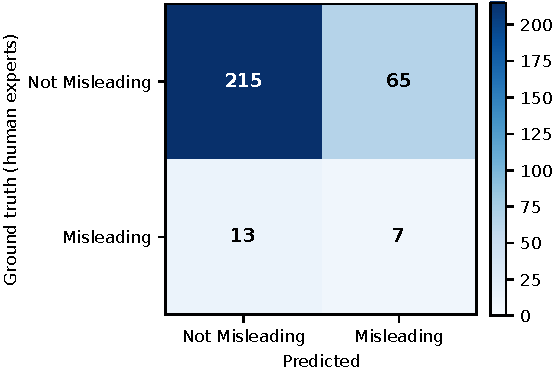
\includegraphics[width=0.75\textwidth]{figures/confusion_matrix_misleading.pdf}
\caption{Confusion matrix for Misleading-argument detection, CoT verifier with context (single run, temperature 0, $n=300$).}
\label{fig:confmat}
\end{figure}
\section{Discussion and Error Analysis}
\label{sec:discussion}
\subsection{Why Does Context Matter So Much?}
The magnitude of the context-availability effect (Table~\ref{tab:context-ablation}) supports our framing in Section~\ref{sec:relwork}: without context, the Verifier's task degrades from grounded fact-checking to something closer to unsupported plausibility judgment, which is a substantially harder and less reliable task for an LLM. This has a direct practical implication for anyone deploying a similar verifier in a real DR-generation pipeline: the original problem context must be retained and passed to the verification stage, not just the generated rationale text.
\subsection{Why Is Misleading Detection Still Hard?}
Even in the best condition (few-shot, with context), Misleading-detection F1 is only 0.188, far below the near-ceiling performance on Helpful (F1 up to 0.997 --- itself partly an artifact of Helpful's 100\% ground-truth base rate, which guarantees perfect precision; see Section~\ref{sec:results}). Three factors plausibly contribute. First, severe class imbalance: only 6.7\% of DRs in our sample contain a Misleading argument (matching Zhou et al.'s reported per-argument rate of 1.59--3.24\%, though note this is not a directly comparable statistic --- our rate is a per-DR \emph{presence} rate while theirs is a per-\emph{argument} rate; a DR can contain one Misleading argument among several correct ones). A rare, high-stakes category is intrinsically harder to achieve high precision on with limited data. Second, the Verifier's precision is consistently low (0.097--0.118 with context) while recall is comparatively higher (0.350--0.550), indicating the Verifier is not conservative --- it flags many arguments as Misleading that are not, trading precision for recall. This is arguably the safer failure mode for a pre-deployment filter (false positives waste a reviewer's time; false negatives let a wrong claim through), but it does mean the Verifier cannot be used to auto-reject DR without human review of the flagged cases. Third, chain-of-thought prompting, which we expected to help most on a task requiring multi-step verification, in fact performs \emph{worst} on Misleading detection among the three strategies (F1 0.152 vs.\ 0.188--0.190). We do not have a confirmed explanation for this; one plausible hypothesis is that explicit step-by-step reasoning makes the Verifier more willing to construct a plausible-sounding chain of justification for \emph{why} an ambiguous argument might be correct, effectively talking itself out of flagging borderline cases that the more direct zero-shot and few-shot prompts still catch. This should be treated as an observation for future investigation rather than a settled explanation, and we did not run repeated trials with resampling to establish its statistical robustness (see Limitations).
\subsection{Confound: DR Length}
Breaking down Misleading-detection performance for the primary condition (CoT, with context) by DR length quartile (Table~\ref{tab:length-quartile}) shows no clean monotonic trend with length. The shortest quartile (Q1, $n=75$, only 3 ground-truth Misleading DRs) achieves \textbf{precision $=$ recall $=$ 0.0}: the Verifier raises 16 false positives in this quartile but catches none of the 3 true positives, effectively guessing rather than over-flagging in a targeted way. Performance peaks in Q2 (F1 $=$ 0.370, the largest ground-truth subgroup at 9 positives) and degrades again in Q3 and Q4. False-positive counts also do \emph{not} decrease with length (16, 13, 14, and 22 in Q1--Q4 respectively) --- if anything the longest quartile produces the most false positives, the opposite of a simple ``over-flags short DRs'' story. Given ground-truth positive counts of only 3--9 per quartile, we treat this breakdown as descriptive rather than as evidence of a specific, generalizable length effect; a larger benchmark would be needed to determine whether DR length is a genuine confound or whether these differences are noise given the small positive counts involved.
\begin{table}[t]
\centering
\caption{Misleading-detection performance by generated-DR length quartile (word count), CoT verifier with context. Q1 = shortest DRs, Q4 = longest. GT+ = number of ground-truth Misleading DRs in the quartile.}
\label{tab:length-quartile}
\begin{tabular}{lccccc}
\toprule
Length quartile & $n$ & GT+ & P & R & F1 \\
\midrule
Q1 (shortest) & 75 & 3 & 0.000 & 0.000 & 0.000 \\
Q2            & 75 & 9 & 0.278 & 0.556 & 0.370 \\
Q3            & 76 & 5 & 0.067 & 0.200 & 0.100 \\
Q4 (longest)  & 74 & 3 & 0.043 & 0.333 & 0.077 \\
\bottomrule
\end{tabular}
\end{table}
\subsection{Confound: Architecture Decision Type}
Performance also varies considerably across Zhou et al.'s architecture-decision-type categories (Table~\ref{tab:decision-type}), though several subgroups are too small ($n<20$ or GT+ $\leq 2$) to support strong conclusions. Table~\ref{tab:decision-type} totals $n=297$, not 300: three DRs are excluded because their source problem's decision-type field in Zhou et al.'s public dataset is a malformed placeholder entry (``IntegrationDecision (example)''), not one of the eight canonical categories, so we cannot assign them a type. Design Pattern Decisions (GT+ $=0$) and Data Decisions (GT+ $=1$) show 0 recall and 0 precision for Misleading in our sample, consistent with having essentially no ground-truth positives to detect, while Integration (GT+ $=1$) and Technology (GT+ $=2$) Decisions show recall of 1.0 on very small positive counts --- a single correct catch out of one or two positives, which should not be read as evidence of a robust detection advantage on those types. We report this breakdown primarily to be transparent about where the Verifier's behavior is (and is not) well-characterized by our sample size, rather than to draw strong per-category conclusions.
\begin{table}[t]
\centering
\caption{Misleading-detection performance by architecture-decision type, CoT verifier with context. GT+ = number of ground-truth Misleading DRs in the type. Subgroups with $n<20$ (marked $^\dagger$) are likely too small for stable estimates.}
\label{tab:decision-type}
\begin{tabular}{lccccc}
\toprule
Decision type & $n$ & GT+ & P & R & F1 \\
\midrule
Architecture Pattern & 36 & 6 & 0.167 & 0.167 & 0.167 \\
Component & 33 & 1 & 0.000 & 0.000 & 0.000 \\
Data & 36 & 1 & 0.000 & 0.000 & 0.000 \\
Deployment$^\dagger$ & 15 & 2 & 0.000 & 0.000 & 0.000 \\
Design Pattern$^\dagger$ & 18 & 0 & 0.000 & 0.000 & 0.000 \\
Implementation & 75 & 7 & 0.150 & 0.429 & 0.222 \\
Integration & 39 & 1 & 0.200 & 1.000 & 0.333 \\
Technology & 45 & 2 & 0.143 & 1.000 & 0.250 \\
\bottomrule
\end{tabular}
\end{table}
\section{Limitations}
\label{sec:limitations}
Our evaluation has several limitations. First, following the constraints of the publicly released ground truth, we evaluate at a \emph{per-DR aggregate} granularity (category presence) rather than a per-argument granularity; a more fine-grained evaluation would require new expert-labeled per-argument ground truth, which is left to future work. Second, all 1{,}200 predictions use a single verifier model (\texttt{gemini-3.1-flash-lite}), chosen for cost and reproducibility reasons under free-tier API constraints rather than because it is necessarily the strongest available judge model; results may not generalize to larger or differently-trained verifier models. Third, although we fix temperature to 0 for reproducibility, we run each condition only once rather than across multiple independent trials, so we cannot report variance estimates or confidence intervals on our F1/Kappa figures; LLM outputs are not perfectly deterministic even at temperature 0, and multi-run replication is recommended before treating any single point estimate (particularly the chain-of-thought under-performance observed in Section~\ref{sec:discussion}) as conclusive. Fourth, our benchmark inherits Zhou et al.'s 100-problem sample size, and the Misleading category in particular has a low base rate (6.7\% of DRs in our per-DR framing), so per-category confound breakdowns (Section~\ref{sec:discussion}) are based on small subgroup sample sizes and should be read as suggestive rather than definitive. Fifth, our context-availability ablation (RQ2) was only run for the chain-of-thought verifier; we do not know whether context matters to the same degree for zero-shot or few-shot prompting, since the interaction between prompting strategy and context availability was not measured. Sixth, Zhou et al.\ do not report inter-annotator agreement for their four human experts' IHUM labeling, so we cannot compare our Verifier's agreement with human ground truth against a human-human agreement ceiling; a low Verifier Kappa could reflect either a weak verifier or an intrinsically difficult, low-agreement labeling task, and we cannot distinguish between these with the information currently available. Finally, our Verifier Agent is a prompt-engineered LLM pipeline rather than a trained or fine-tuned classifier; we view this as a deliberate design choice (zero additional training cost, immediate applicability to any DR-generation pipeline) but note it likely leaves detection accuracy on the table compared to an approach with dedicated training data.
\section{Conclusion}
\label{sec:conclusion}
We presented, to our knowledge, the first empirical evaluation of an LLM-based Verifier Agent for automatically detecting Misleading design rationale generated by LLMs for software architecture decisions, extending Zhou et al.'s manually-labeled benchmark with an automated, reproducible labeling pipeline. Across 1{,}200 verifier predictions spanning three prompting strategies and a context-availability ablation, we find that providing the Verifier Agent with the original architecture-problem context is --- at least for the chain-of-thought verifier, the only strategy for which we measured this effect --- far more important than the choice of prompting strategy, nearly tripling Misleading-detection F1 (0.056 $\rightarrow$ 0.152) and substantially raising overall macro-F1 (0.406 $\rightarrow$ 0.608). At the same time, Misleading detection remains a hard, low-precision task even in the best configuration (F1 0.188), and our error analysis finds no clean relationship between Misleading-detection accuracy and DR length, and shows the Verifier struggles disproportionately on some architecture-decision types. We conclude that an LLM Verifier Agent is a promising, zero-training-cost \emph{first line of defense} for flagging DR for human review, rather than a drop-in replacement for expert judgment, and we release our prompts, code, and full API call logs to support replication and extension.
\subsubsection*{Code and Data Availability}
Our Verifier Agent implementation, all prompts (zero-shot, chain-of-thought, few-shot), evaluation scripts, the full API call log (including the resolved model version for every call), and the two additional ablation figures not embedded in this paper for space reasons (\texttt{ablation\_context.png}, \texttt{ablation\_prompt\_variant.png} --- both visualizing data already reported in Tables~\ref{tab:context-ablation} and~\ref{tab:prompt-ablation}) are available at \url{https://github.com/phatom2005/Automating-the-Detection-of-Misleading-Design-Rationale-Generated-by-Large-Language-Models}. We use the publicly available LLM4DR dataset and ground-truth labels from Zhou et al.\ \cite{zhou2025llm} without modification.
\subsubsection*{Acknowledgments}
The authors would like to thank Le Nguyen Son Vu for his valuable guidance and constructive feedback throughout the development of this study.
\subsubsection*{Disclosure of Interests}
The authors have no competing interests to declare that are relevant to the content of this article. For disclosure of AI assistance used in preparing this manuscript, see Section~\ref{sec:methodology}.
\begin{thebibliography}{8}
\bibitem{zhou2025llm}
Zhou, X., Li, R., Liang, P., Zhang, B., Shahin, M., Li, Z., Yang, C.:
Using LLMs in Generating Design Rationale for Software Architecture Decisions.
ACM Transactions on Software Engineering and Methodology (TOSEM) (2025).
\url{https://arxiv.org/abs/2504.20781}
\bibitem{zheng2023judging}
Zheng, L., Chiang, W.L., Sheng, Y., Zhuang, S., Wu, Z., Zhuang, Y., Lin, Z., Li, Z., Li, D., Xing, E.P., Zhang, H., Gonzalez, J.E., Stoica, I.:
Judging LLM-as-a-Judge with MT-Bench and Chatbot Arena.
In: Advances in Neural Information Processing Systems (NeurIPS), Datasets and Benchmarks Track (2023).
\url{https://arxiv.org/abs/2306.05685}
\bibitem{dhar2024llm}
Dhar, R., Vaidhyanathan, K., Varma, V.:
Can LLMs Generate Architectural Design Decisions? -- An Exploratory Empirical Study.
In: IEEE International Conference on Software Architecture (ICSA) (2024).
\url{https://arxiv.org/abs/2403.01709}
\bibitem{diazpace2024archmind}
D\'{i}az-Pace, J.A., Tommasel, A., Capilla, R.:
Helping Novice Architects to Make Quality Design Decisions Using an LLM-Based Assistant.
In: Software Architecture (ECSA 2024). LNCS, vol.\ 14889. Springer, Cham (2024).
\url{https://doi.org/10.1007/978-3-031-70797-1_21}
\bibitem{huang2025survey}
Huang, L., Yu, W., Ma, W., Zhong, W., Feng, Z., Wang, H., Chen, Q., Peng, W., Feng, X., Qin, B., Liu, T.:
A Survey on Hallucination in Large Language Models: Principles, Taxonomy, Challenges, and Open Questions.
ACM Transactions on Information Systems (TOIS) 43(2) (2025).
\url{https://arxiv.org/abs/2311.05232}
\bibitem{farquhar2024semantic}
Farquhar, S., Kossen, J., Kuhn, L., Gal, Y.:
Detecting Hallucinations in Large Language Models Using Semantic Entropy.
Nature 630(8017), 625--630 (2024).
\url{https://doi.org/10.1038/s41586-024-07421-0}
\bibitem{manakul2023selfcheckgpt}
Manakul, P., Liusie, A., Gales, M.J.F.:
SelfCheckGPT: Zero-Resource Black-Box Hallucination Detection for Generative Large Language Models.
In: Proceedings of EMNLP 2023, pp.\ 9004--9017 (2023).
\url{https://arxiv.org/abs/2303.08896}
\bibitem{alhoshan2025requirements}
Alhoshan, W., Ferrari, A., Zhao, L.:
How Effective are Generative Large Language Models in Performing Requirements Classification?
arXiv preprint (2025). \url{https://arxiv.org/abs/2504.16768}
\end{thebibliography}
\end{document}
